% questions.tex —— 2019 年·上海春季招生数学试卷 · 题目内容片段（无答案）
% 由 tools/generate_projects.py 依来源总账自 2019/2019_数学真题_春季上海_试题.md 生成，勿手改（改源 MD 后重跑）


\begin{gktip}
\textbf{来源边界}：题签文字取自固定 PDF。该 15 页文件的第 1–3 页是题面，第 4–15 页自称参考答案和解析；出版者、版次、官方身份及其与正式原卷的对应关系尚未核实。题稿已由第二位复核者对照固定副本逐题核对；源内疑点仍待核，文件没有提供可确认的每题分值。源附答案仅作摘录，未视为官方答案。

\textbf{题图}：第 10、17 题已按固定 PDF 页图重绘为 TikZ 矢量图，比例为示意；图稿已局部编译，并由主会话对照源图复核，正式排版验收仍待完成。第 16 题源附答案与严格轨迹存在疑点，见摘录和 intake 报告。
\end{gktip}

\gkpart{一、填空题}

\begin{question}
\gkti{1}已知集合 $A=\{1,2,3,4,5\}$，$B=\{3,5,6\}$，则 $A\cap B=\underline{\qquad\qquad}$。（PDF 第 1 页）

\end{question}
\begin{question}
\gkti{2}计算 $\displaystyle\lim_{n\to\infty}\frac{2n^2-3n+1}{n^2-4n+1}=\underline{\qquad\qquad}$。（PDF 第 1 页）

\end{question}
\begin{question}
\gkti{3}不等式 $|x+1|<5$ 的解集为 $\underline{\qquad\qquad}$。（PDF 第 1 页）

\end{question}
\begin{question}
\gkti{4}函数 $f(x)=x^2\ (x>0)$ 的反函数为 $\underline{\qquad\qquad}$。（PDF 第 1 页）

\end{question}
\begin{question}
\gkti{5}设 $i$ 为虚数单位，$3\overline z-i=6+5i$，则 $|z|$ 的值为 $\underline{\qquad\qquad}$。（PDF 第 1 页）

\end{question}
\begin{question}
\gkti{6}已知 $\begin{cases}2x+2y=-1,\\4x+a^2y=a,\end{cases}$ 当方程有无穷多解时，$a$ 的值为 $\underline{\qquad\qquad}$。（PDF 第 1 页）

\end{question}
\begin{question}
\gkti{7}在 $\left(x+\dfrac{1}{\sqrt{x}}\right)^6$ 的二项展开式中，常数项的值为 $\underline{\qquad\qquad}$。（PDF 第 1 页）

\end{question}
\begin{question}
\gkti{8}在 $\triangle ABC$ 中，$AC=3$，$3\sin A=2\sin B$，且 $\cos C=\dfrac14$，则 $AB=\underline{\qquad\qquad}$。（PDF 第 1 页）

\end{question}
\begin{question}
\gkti{9}首届中国国际进口博览会在上海举行，某高校拟派 4 人参加连续 5 天的志愿者活动，其中甲连续参加 2 天，其他人各参加 1 天，则不同的安排方法有 $\underline{\qquad}$ 种（结果用数值表示）。（PDF 第 1 页）

\begin{gktip}
待核：固定副本未显式说明五天是否每天都须有人参加；不同解释会影响计数。
\end{gktip}

\Needspace{0.4\textheight}
\end{question}
\begin{question}
\gkti{10}如图，已知正方形 $OABC$，其中 $OA=a\ (a>1)$，函数 $y=3x^2$ 交 $BC$ 于点 $P$，函数 $y=x^{-\frac12}$ 交 $AB$ 于点 $Q$，当 $|AQ|+|CP|$ 最小时，则 $a$ 的值为 $\underline{\qquad\qquad}$。（PDF 第 1 页）
\nopagebreak[4]
\begin{center}% 2019 上海春季卷第 10 题；取 a=2 作示意，曲线、交点依题设计算。
% 图形比例为排版示意，不对应源图物理尺寸。
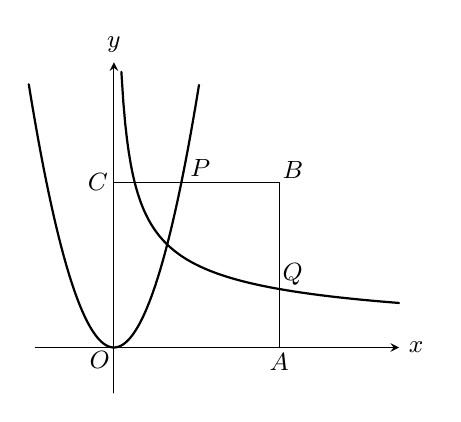
\begin{tikzpicture}[x=1.05cm,y=1.05cm,line cap=round,line join=round,>=stealth,font=\small]
  \coordinate (O) at (0,0);
  \coordinate (A) at (2,0);
  \coordinate (B) at (2,2);
  \coordinate (C) at (0,2);
  \coordinate (P) at ({sqrt(2/3)},2);
  \coordinate (Q) at (2,{1/sqrt(2)});

  \draw[->] (-0.95,0) -- (3.45,0) node[right] {$x$};
  \draw[->] (0,-0.55) -- (0,3.45) node[above] {$y$};
  \draw (C) -- (B) -- (A);
  \draw[thick,domain=-1.03:1.03,samples=90] plot (\x,{3*\x*\x});
  \draw[thick,domain=0.09:3.45,samples=150] plot (\x,{1/sqrt(\x)});

  \node[below left,inner sep=1.3pt] at (O) {$O$};
  \node[below,inner sep=2pt] at (A) {$A$};
  \node[above right,inner sep=1pt] at (B) {$B$};
  \node[left,inner sep=2pt] at (C) {$C$};
  \node[above right,xshift=2pt,yshift=1pt,inner sep=1pt] at (P) {$P$};
  \node[above right,inner sep=1pt] at (Q) {$Q$};
\end{tikzpicture}
\end{center}
\nopagebreak[4]
\end{question}
\begin{question}
\gkti{11}在椭圆 $\dfrac{x^2}{4}+\dfrac{y^2}{2}=1$ 上任意一点 $P$，$Q$ 与 $P$ 关于 $x$ 轴对称，若有 $\overrightarrow{F_1P}\cdot\overrightarrow{F_2P}\leq1$，则 $\overrightarrow{F_1P}$ 与 $\overrightarrow{F_2Q}$ 的夹角范围为 $\underline{\qquad\qquad}$。（PDF 第 1 页）

\begin{gktip}
待核：固定副本题干未显式定义 $F_1,F_2$；不能仅凭记号补写定义。
\end{gktip}

\end{question}
\begin{question}
\gkti{12}已知集合 $A=[t,t+1]\cup[t+4,t+9]$，$0\notin A$，存在正数 $\lambda$，使得对任意 $a\in A$，都有 $\dfrac{\lambda}{a}\in A$，则 $t$ 的值是 $\underline{\qquad\qquad}$。（PDF 第 1 页）

\end{question}
\gkpart{二、单选题}

\begin{question}
\gkti{13}下列函数中，值域为 $[0,+\infty)$ 的是\mbox{（　　）}。（题干 PDF 第 1 页，选项第 2 页）

（A）$y=2^x$　　（B）$y=x^{\frac12}$　　（C）$y=\tan x$　　（D）$y=\cos x$

\end{question}
\begin{question}
\gkti{14}已知 $a,b\in\mathbb R$，则“$a^2>b^2$”是“$|a|>|b|$”的\mbox{（　　）}。（PDF 第 2 页）

（A）充分非必要条件　　（B）必要非充分条件

（C）充要条件　　（D）既非充分又非必要条件

\end{question}
\begin{question}
\gkti{15}已知平面 $\alpha,\beta,\gamma$ 两两垂直，直线 $a,b,c$ 满足 $a\subset\alpha$，$b\subset\beta$，$c\subset\gamma$，则直线 $a,b,c$ 不可能满足以下哪种关系\mbox{（　　）}。（PDF 第 2 页）

（A）两两垂直　　（B）两两异面　　（C）两两相交　　（D）两两平行

\end{question}
\begin{question}
\gkti{16}以 $(a_1,0),(a_2,0)$ 为圆心的两圆均过 $(1,0)$，与 $y$ 轴正半轴分别交于 $(0,y_1),(0,y_2)$，且满足 $\ln y_1+\ln y_2=0$，则点 $\left(\dfrac1{a_1},\dfrac1{a_2}\right)$ 的轨迹是\mbox{（　　）}。（PDF 第 2 页）

（A）直线　　（B）圆　　（C）椭圆　　（D）双曲线

\end{question}
\gkpart{三、解答题}

\Needspace{0.4\textheight}
\begin{question}
\gkti{17}如图，在正三棱锥 $P-ABC$ 中，$PA=PB=PC=2$，$AB=BC=AC=\sqrt3$。（PDF 第 2 页）

（1） 若 $PB$ 的中点为 $M$，$BC$ 的中点为 $N$，求 $AC$ 与 $MN$ 的夹角；

（2） 求 $P-ABC$ 的体积。
\nopagebreak[4]
\begin{center}% 2019 上海春季卷第 17 题；透视投影为示意，M、N 按两条线段中点构造。
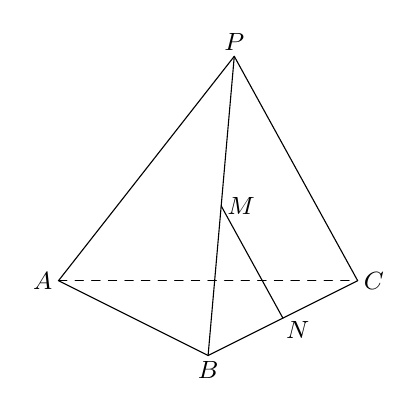
\begin{tikzpicture}[scale=0.95,line cap=round,line join=round,font=\small]
  \coordinate (A) at (0,1);
  \coordinate (B) at (2,0);
  \coordinate (C) at (4,1);
  \coordinate (P) at (2.35,4);
  \coordinate (M) at (2.175,2);
  \coordinate (N) at (3,0.5);

  \draw[dashed] (A) -- (C);
  \draw (P) -- (A) -- (B) -- (C) -- cycle;
  \draw (P) -- (B);
  \draw (M) -- (N);

  \node[left,inner sep=2pt] at (A) {$A$};
  \node[below,inner sep=2pt] at (B) {$B$};
  \node[right,inner sep=2pt] at (C) {$C$};
  \node[above,inner sep=2pt] at (P) {$P$};
  \node[right,inner sep=2pt] at (M) {$M$};
  \node[below right,inner sep=1pt] at (N) {$N$};
\end{tikzpicture}
\end{center}
\nopagebreak[4]
\end{question}
\begin{question}
\gkti{18}已知数列 $\{a_n\}$，$a_1=3$，前 $n$ 项和为 $S_n$。（PDF 第 2 页）

（1） 若 $\{a_n\}$ 为等差数列，且 $a_4=15$，求 $S_n$；

（2） 若 $\{a_n\}$ 为等比数列，且 $\displaystyle\lim_{n\to\infty}S_n<12$，求公比 $q$ 的取值范围。

\end{question}
\begin{question}
\gkti{19}已知抛物线方程 $y^2=4x$，$F$ 为焦点，$P$ 为抛物线准线上一点，$Q$ 为线段 $PF$ 与抛物线的交点，定义：$d(P)=\dfrac{|PF|}{|FQ|}$。（PDF 第 2–3 页）

（1） 当 $P\left(-1,-\dfrac83\right)$ 时，求 $d(P)$；

（2） 证明：存在常数 $a$，使得 $2d(P)=|PF|+a$；

（3） $P_1,P_2,P_3$ 为抛物线准线上三点，且 $|P_1P_2|=|P_2P_3|$，判断 $d(P_1)+d(P_3)$ 与 $2d(P_2)$ 的关系。

\end{question}
\begin{question}
\gkti{20}已知等差数列 $\{a_n\}$ 的公差 $d\in(0,\pi]$，数列 $\{b_n\}$ 满足 $b_n=\sin(a_n)$，集合 $S=\{x\mid x=b_n,\ n\in\mathbb N^*\}$。（PDF 第 3 页）

（1） 若 $a_1=0$，$d=\dfrac{2\pi}{3}$，求集合 $S$；

（2） 若 $a_1=\dfrac\pi2$，求 $d$ 使得集合 $S$ 恰好有两个元素；

（3） 若集合 $S$ 恰好有三个元素：$b_{n+T}=b_n$，$T$ 是不超过 7 的正整数，求 $T$ 的所有可能的值。

\end{question}